%% grundlagen.tex
%% $Id: grundlagen.tex 28 2007-01-18 16:31:32Z bless $
%%

\chapter{Grundlagen}
\label{ch:Grundlagen}
%% ==============================

%% ==============================
\section{Kryptographie mit öffentlichen Schlüsseln}
%% ==============================
\label{ch:Grundlagen:sec:PublicKeyCrypto}

\subsection{Prinzip}
\label{ch:Grundlagen:sec:PublicKeyCrypto:subsec:Prinzip}

Klassische Kryptographie basiert auf einem \emph{Geheimnis} oder
\emph{privaten Schl\"ussel}, der beiden Kommunikationspartnern bekannt
ist. 

\subsection{Authentisierung von Schlüsseln}
\label{ch:Grundlagen:sec:PublicKeyCrypto:subsec:KeyAuth}

Zweck von PKI oder Web of Trust ist es, die Authentizit\"at der
Bindung von Schl\"ussel/Zertifikat und Identit\"at zu etablieren. Und
das eben auch dann, wenn man selbst diese Bindung nicht \"uberpr\"ufen
kann.

\subsubsection{Zentrale PKI}
\label{ch:Grundlagen:sec:PublicKeyCrypto:subsec:KeyAuth:subsubsec:PKI}

\subsubsection{Web of Trust}
\label{ch:Grundlagen:sec:PublicKeyCrypto:subsec:KeyAuth:subsubsec:WOT}

\section{PGP/GnuPG}
\label{ch:Grundlagen:sec:PGP}

\subsection{Geschichte von PGP und GnuPG}
\label{ch:Grundlagen:sec:PGP:subsec:Geschichte}

\subsection{Eigenschaften/Fähigkeiten der Implementierungen}
\label{ch:Grundlagen:sec:PGP:subsec:Eigenschaften}

\subsection{Das GnuPG-Vertrauensmodell}
\label{sec:das-gnupg-vertrauensmodell}

Öffentliche PGP-Schlüssel werden oft nicht in einer Weise übergeben,
die die sofortige Verifikation des Schlüssels zulässt, beispielsweise
bei einem persönlichen Treffen. Stattdessen werden Schlüssel häufig
per E-Mail, über einen Keyserver oder andere elektronische Wege
ausgetauscht.  Überprüfung der Authentizität eines Schlüssels ist
deswegen von grosser Bedeutung.

Ein Schlüssel wird von GnuPG genau dann als gültig (\emph{valid})
betrachtet, wenn er die folgenden Bedingungen erfüllt:

\begin{enumerate}
\item Der Schlüssel wurde von ausreichend vielen \emph{gültigen} Schlüsseln
  unterschrieben, d.h. er wurde mindestens entweder von
  \begin{itemize}
  \item dem Besitzer des Schlüsselrings selbst (d.h. von einem
    Schlüssel mit \emph{ultimate trust}) unterschrieben
  \item mindestens $N$ gültigen Schlüsseln, denen voll vertraut wird, unterschrieben
  \item mindestens $M$ gültigen Schlüsseln, denen geringfügig
    vertraut wird, unterschrieben
  \end{itemize}
\item Eine Signaturkette wird nur verwendet, wenn sie ausgehend vom
  Besitzer des Schlüsselrings maximal die Länge $L$ hat.
\end{enumerate}

Ein Schlüssel, der von weniger voll bzw. geringfügig
vertrauenswürdigen Schlüsseln als notwendig unterschrieben wurde, wird
als eingeschränkt gültig (\emph{marginally valid})
angesehen. Allerdings werden Schlüssel dieser Kategorie von GnuPG
genauso wie nicht gültige Schlüssel behandelt.

GnuPG verwendet in der Standardeinstellung die Werte $N=1$, $M=3$ und
$L=5$. Damit wird \emph{ein} Zertifikat, dass von einem Schl\"ussel
mit vollem Vertrauen ausgestellt wurde, als ausreichend
betrachtet. F\"ur Schl\"ussel, denen nur geringf\"ugig vertraut wird,
ist ein einzelnes Zertifikat nicht ausreichend. Dieses muss noch durch
2 weitere solche Zertifikate best\"atigt werden. 

GnuPG erlaubt es einem Anwender, die Parameter $N, M$ und $L$ selbst
zu setzen und damit seine Sicherheitsanforderungen umzusetzen. Je
höher beispielsweise die notwendige Anzahl von Signaturen, um so
kleiner ist der Schaden, den eine einzelne fehlerhafte Signatur
anrichten kann. Ist die maximale Pfadlänge auf einen kleinen Wert
begrenzt, so ist auch die maximale Anzahl der Signaturen auf dem Pfad
kleiner, die potentiell fehlerhaft sein können. Andererseits
verringert sich damit die Anzahl der Signaturen (Pfade im Web of
Trust), die für die Verifizierung benutzt werden können, und damit die
Anzahl verifizierbarer Schlüssel. Es muss also eine Abwägung zwischen
dem Sicherheitsbedürfnis des Nutzers und der praktischen Benutzbarkeit
getroffen werden.

\begin{figure}[t]
  \centering
  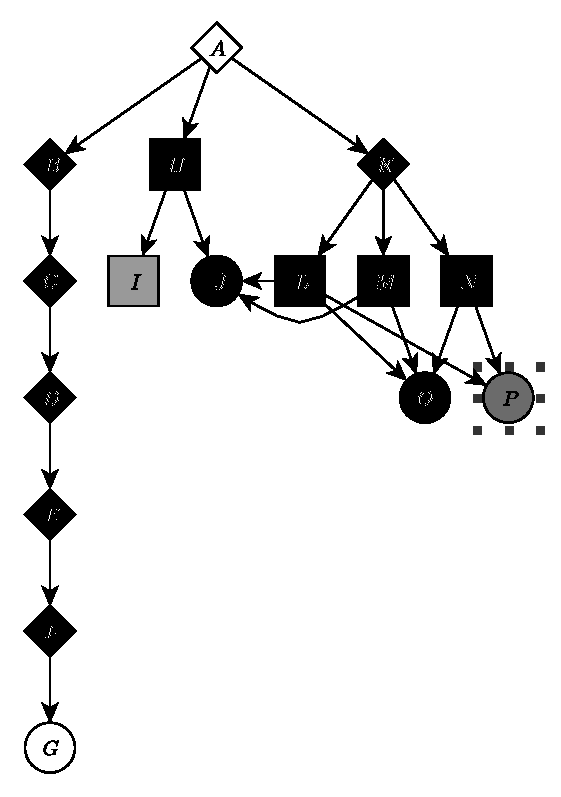
\includegraphics[scale=1.0]{images/trust-beispiel.pdf}
  \caption{Beispiel für die Berechnung der Gültigkeit von Schlüsseln}
  \label{fig:trust-beispiel}
\end{figure}

Abbildung \ref{fig:trust-beispiel} gibt ein Beispiel für die
Berechnung der Schlüsselgültigkeit unter Verwendung der
Standard-Parameter $N=1$, $M=3$ und $L=5$. Die Schlüssel $B, H$ und
$K$ wurden direkt von $A$, dem Besitzer des Schlüsselrings,
unterschrieben und sind deshalb voll gültig. Da $L, M,$ und $N$ von
$K$ unterschrieben wurden und dieser über volles Vertrauen verfügt,
sind sie ebenfalls voll gültig. $O$ sowie $J$ sind voll gültig, da sie
jeweils von drei Schlüsseln mit geringfügigem Vertrauen unterschrieben
wurden. $I$ und $P$ wurden dagegen jeweils nur von zwei Schlüsseln mit
geringfügigem Vertrauen unterschrieben und sind deshalb nicht voll
sondern nur eingeschränkt gültig. $G$ wurde zwar von einem voll
gültigen Schlüssel mit vollem Vertrauen unterschrieben. Allerdings
überschreitet die Signaturkette zu $A$ die maximale Länge von 5 und
wird deshalb nicht betrachtet.

Ein öffentlicher Schlüssel, der anhand dieser Regeln nicht als
authentisch verifiziert werden kann, kann trotzdem zur Verschlüsselung
und zur Verifizierung von Signaturen verwendet werden. Allerdings
warnt GnuPG in diesem Fall vor der Verwendung.

\subsection{Soziale Komponente des Web of Trust}
\label{sec:sozi-komp-des}

PGP-CAs (CACert?, CT) erwaehnen, Crypto-Kampagne der CT

In einer Reihe von Open-Source-Projekten spielen PGP und das Web of
Trust eine wichtige Rolle. Im Debian-Projekt beispielweise werden
PGP-Schl\"ussel unter anderem benutzt, um alle bereitgestellten
Softwarepakete durch den zust\"andigen Entwickler signieren zu
lassen. Dazu muss jeder Debian-Entwickler \"uber einen Schl\"ussel
verf\"ugen, der von mindestens einem anderen Debian-Entwickler
verifiziert und unterschrieben wurde. Auf diese Weise bildet sich
bereits innerhalb des Projekts ein Web of Trust. PGP scheint eine
wichtige Rolle in der Kultur des Projekts zu spielen. 



%% ==============================
\section{Der OpenPGP-Standard (RFC4880)}
%% ==============================
\label{ch:Grundlagen:sec:OpenPGP}

\subsection{Paketformat v4}
\label{ch:Grundlagen:sec:OpenPGP:subsec:PaketFormat}

\subsection{Unterschiede v3}
\label{ch:Grundlagen:sec:OpenPGP:subsec:v3Format}

\section{Graphentheorie allgemein}
\label{ch:Grundlagen:sec:Graphentheorie}

\section{Netzwerkanalyse}
\label{ch:Grundlagen:sec:Netzwerkanalyse}

\subsection{Netzwerkstatistiken}
\label{ch:Grundlagen:sec:Netzwerkanalyse:subsec:Statistiken}

\subsection{Communities}
\label{ch:Grundlagen:sec:Netzwerkanalyse:subsec:Communities}

\subsection{Modularity}
\label{sec:modularity}

\begin{equation}
  \label{eq:modularity}
  Q =
  \frac{1}{2m}\sum_{ij}\left(A_{ij}-\frac{d_id_j}{2m}\right)\delta(c_i, c_j)
\end{equation}

Seit der Arbeit von Newman wurde eine Vielzahl weiterer Methoden zur
Erkennung von Communities vorgestellt. An dieser Stelle werden 3
Methoden n\"aher beschrieben, die in dieser Arbeit verwendet
werden. Einen Gesamt\"uberblick bietet ein \"Ubersichtsartikel von
Fortunato \cite{Fortunato2010}.

%% ==============================
\section{Verwandte Arbeiten}
%% ==============================
\label{ch:Grundlagen:sec:RelatedWork}

\subsection{Analysen des OpenPGP-Web of Trust}
\label{ch:Grundlagen:sec:RelatedWork:subsec:wot-analysis}

\subsection{Community-Strukturen allgemein}
\label{ch:Grundlagen:sec:RelatedWork:subsec:community-analysis}
%%% Local Variables: 
%%% mode: latex
%%% TeX-master: "diplarb"
%%% End: 
